% Este arquivo .tex será incluído no arquivo .tex principal. Não é preciso
% declarar nenhum cabeçalho

\section{Lugares para morar}

O preço de uma casa é a área do paralelepípedo formado pelos seguintes valores
nos eixos: proximidade da Unicamp, tamanho da casa (quantidade de quartos)
e qualidade da casa (acabamento, quantidade de banheiros, etc.) Quanto
à distância, a avenida 1 (avenida Dr. Romeu Tórtima) e avenida 2 (avenida Prof.
Atílio Martini) são bem caras por serem próximas da Unicamp, as ruas entre elas
muitas vezes também são. A região que vai do centro de Barão até a moradia
geralmente é boa e barata para se morar: Tem bastantes serviços e ainda é perto
da Unicamp (mais ou menos 10 minutos de bicicleta).

Uma boa dica para se informar a respeito de lugares para morar (repúblicas,
kitnets, pensões) é o site Morar Unicamp
(\url{www.morarunicamp.com.br}), criado por alunos da Unicamp e que
contém informações como endereço, preço, contato e detalhamento do lugar. E mais
lugares podem ser adicionados ao site.

\subsection{Moradia Estudantil}

A moradia estudantil é um exemplo de conquista de todos os estudantes.
O processo de reivindicação de uma moradia estudantil para a Unicamp começou com
o movimento TABA. Durante muito tempo, alunos ficaram acampados no CB (Ciclo
Básico) para reivindicar seu direito a estudar.
\begin{figure}[h!]
    \centering
    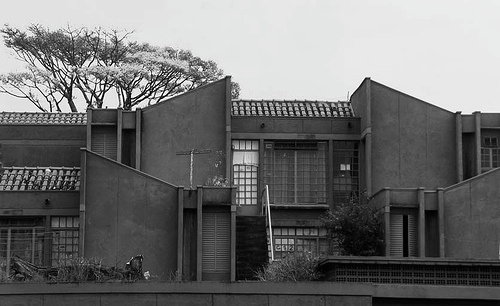
\includegraphics[scale=0.55,keepaspectratio=true]{img/imgs/5-moradia/-029.jpg}
\end{figure}
Hoje em dia, graças à moradia,
várias pessoas que possivelmente não teriam condições de se manter em Campinas
pagando aluguel, tem como estudar na Unicamp. A moradia existe desde 1989
e durante esse período a Unicamp ampliou muito suas vagas. Isto fez as vagas na
moradias tornarem-se insuficientes para todos que querem. Alguns anos atrás
houve grandes movimentações pela ampliação e reforma da moradia, pois algumas
casas estavam caindo.

Cada "casa" (que normalmente é dividida entre quatro pessoas) se constitui de um
quarto, uma cozinha, um banheiro e uma sala. Ainda tem o Circular da Moradia, um
ônibus da Unicamp que transporta a galera durante o dia todo da moradia até
a Unicamp e vice-versa.

A moradia está localizada na Avenida Santa Isabel, 1125. Aproximadamente a uns
3 km do campus da Unicamp.

Para saber mais sobre o processo seletivo entre no site da Moradia Estudantil
(\url{www.pme.unicamp.br}). Muito provavelmente você
será abordado por um assistente social na matrícula.

\subsection{Repúblicas}

Geralmente a melhor escolha, se você tiver condições de pagar por uma moradia.
\begin{figure}[h!]
    \vspace{-10pt}
    \centering
    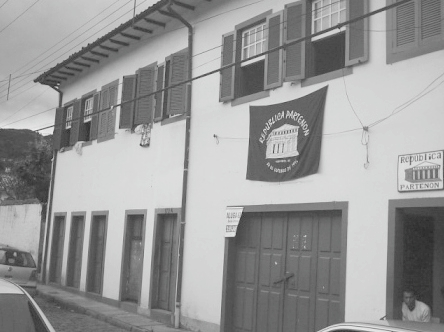
\includegraphics[scale=0.58,keepaspectratio=true]{img/imgs/5-moradia/-034.jpg}
    \vspace{-10pt}
\end{figure}
Você pode levar quem quiser para sua casa (dependendo da aprovação dos
moradores), chegar no horário que quiser, e conhecerá muita gente nova. Tente,
se possível, morar em uma república de cursos mistos, pois assim você terá
contatos diversos. O custo de uma vaga em uma república é muito variável
(depende do nível de conforto que você quer). Gira em torno de
R\$350,00 o aluguel para dividir quarto e R\$450,00 para pegar
um quarto sozinho, além das contas adicionais (água, luz, etc.), que costumam
totalizar R\$150,00, em média. Procure bem as pessoas com quem você vai morar para não ter
problemas com diferentes estilos de vida (tem gente que gosta de lavar louça
a cada 5 minutos e tem gente que gostaria de morar junto com porcos, veja com
quem você se dá melhor).

\subsection{Kitnets}

Tomem cuidado com elas, pois a especulação imobiliária em Barão Geraldo chega
a ser imbecil. E nos últimos anos ficou fora de controle. As kitnets mobiliadas,
normalmente um quarto-sala-cozinha-área de serviço e banheiro, estão com valores
da ordem de R\$ 1000,00 para mais. Sim, mil reais por um microespaço. Só porque
é perto da Unicamp. Fique de olho e tome cuidado com os contratos.
\begin{figure}[h!]
    \centering
    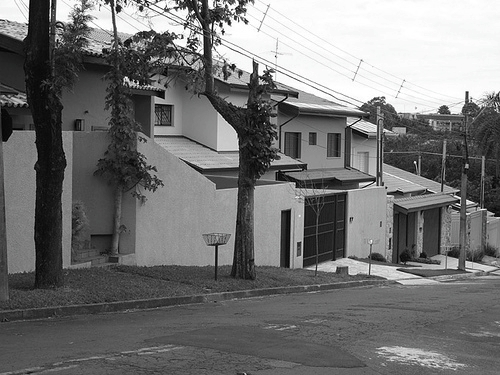
\includegraphics[scale=0.55,keepaspectratio=true]{img/imgs/5-moradia/-033.jpg}
\end{figure}

As melhores relações custo-benefício de kitnets são aquelas próximas ao centro
de Barão Geraldo ou no espaço entre as avenidas. E lembre-se não é só de Unicamp
que se vive. Não adianta pagar mais caro para estar do lado da Unicamp, se você
fica muito longe dos mercados, farmácias etc.

\subsection{Pensões}

Dependendo da pensão que você conseguir pode tornar-se uma grande roubada.
Algumas pensões não deixam você levar pessoas para sua casa, reclamam se você
chegar tarde e não liberam festas, já outras não; então procure bem. O preço
também não é muito bom, mas costuma ser mais barato que kitnets. É bom se você
quer um esquema casa-comida-roupa-lavada. É muito importante que você saiba que
contratos de um ano (ou qualquer período) em pensionatos são ilegais e você não
precisa cumpri-los.

\subsection{Dicas de Segurança}

Além de um novo ambiente de estudos, conhecerá novos lugares e pessoas. E,
provavelmente, em breve estará planejando sua mudança para Campinas.

Muitos dos estudantes moram em Barão Geraldo, por ser mais perto da Unicamp,
possibilitando que sua bicicleta se torne seu meio de transporte principal, por
ser o lugar com maior número de repúblicas e pensionatos e também por ser onde
a maior parte das festas acontece!

No entanto, por ser constituído em sua maioria por casas de famílias com muitas
posses e casas de estudantes (em geral desatentos), Barão Geraldo peca pela
falta de segurança.

Não é raro ouvir de alguém que foi assaltado enquanto voltava para casa à noite
sozinho ou que a casa foi saqueada durante um feriado prolongado. Portanto,
é importante zelar pela sua integridade e de seus pertences -- assim como seus
pais fazem em sua casa, não importa onde eles morem.
\begin{figure}[h!]
    \centering
    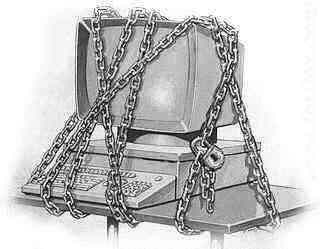
\includegraphics[scale=0.55,keepaspectratio=true]{img/imgs/5-moradia/seguranca.jpg}
\end{figure}

Se sua pensão ou república paga o segurança da rua, faça uso dele, seja pedindo
escolta ao chegar em casa ou telefonando caso ouça algum barulho suspeito. Ao
voltar para sua cidade em feriados prolongados, deixando a casa vazia, não se
esqueça de trancar todas as portas e janelas de casa, verificar se não há nada
no quintal que possa ser levado facilmente (colocar as bicicletas e aparelhos de
som na sala pode ser uma boa ideia), e trancar os objetos de valor
(computadores, televisões) nos quartos.

\subsection{Imobiliárias}

\begin{itemize}
\item  \textbf{Imobiliária Barão Housing}
\begin{itemize}
\item  Telefone: (19)3289-4113.
\item  Endereço: Rua Tranquilo Prosperi, 383 -- Jd. Sta. Genebra II.
\item  E-mail: atendimento [@] baraohousing [.] com[.] br.
\item  Site: \url{www.baraohousing.com.br}
\end{itemize}
\end{itemize}

\begin{itemize}
\item  \textbf{Imobiliária Home Hunters}
\begin{itemize}
\item  Endereço: Rua Benedito Alves Aranha, 55.
\item  Telefone: (19) 3289-0044.
\item  E-mail: bgeraldo [@] homehunters [.] com [.] br.
\item  Site: \url{www.homehunters.com.br}
\end{itemize}
\end{itemize}

\begin{itemize}
\item  \textbf{Imobiliária Barão Geraldo}
\begin{itemize}
\item  Endereço: Aavenida Dr. Romeu Tórtima, 183.
\item  Telefone: (19) 3289-2315.
\item  E-mail: atendimento [@] imobiliariabaraogeraldo [.] com [.] br.
\item  Site: \url{www.imobiliariabaraogeraldo.com.br}
\end{itemize}
\end{itemize}

\begin{itemize}
\item  \textbf{Imobiliária Lanza}
\begin{itemize}
\item  Endereço: Rua Benedito Alves Aranha, 104.
\item  Telefone: (19) 3289-1717.
\item  E-mail: lanza [@] lanzaimoveis [.] com [.] br.
\item  Site: \url{www.lanzaimoveis.com.br}
\end{itemize}
\end{itemize}

\begin{itemize}
\item  \textbf{Imobiliária Professor Sebastião}
\begin{itemize}
\item  Endereço: Avenida Dr. Romeu Tórtima, 344.
\item  Telefone: (19) 3289-2317.
\item  E-mail: ipsimoveis [@] ipsimoveis[.] com [.] br.
\item  Site: \url{www.ipsimoveis.com.br}
\end{itemize}
\end{itemize}

\begin{itemize}
\item  \textbf{Amaral Imóveis}
\begin{itemize}
\item  Endereço: Avenida Dr. Luiz de Tella, 864.
\item  Telefone: (19) 3287-5255.
\item  E-mail: amaral [@] amaralimoveis [.] net.
\item  Site: \url{www.amaralimoveis.net/}
\end{itemize}
\end{itemize}

\begin{itemize}
\item  \textbf{Zaine Conquista Imóveis}
\begin{itemize}
\item  Endereço: Avenida Santa Izabel, 84.
\item  Telefone: (19)3289-4050.
\item  E-mail: zaine [@] correionet [.] com [.] br.
\item  Site: \url{www.zaineconquista.com.br}
\end{itemize}
\end{itemize}

\begin{itemize}
\item  \textbf{W. Post Imóveis}
\begin{itemize}
\item  Endereço: Avenida Dr. Romeu Tórtima, 1140.
\item  Telefone: (19) 3289-2155.
\item  E-mail: w.post [@] ig [.] com [.] br.
\item  Site: \url{www.wpostimoveis.com.br}
\end{itemize}
\end{itemize}

\begin{itemize}
\item  \textbf{Ismê Assessoria Imobiliária}
\begin{itemize}
\item  Endereço: Rua Christina G. Miguel, 250.
\item  Telefone: (19) 3289-4325.
\item  E-mail: isme [@] isme [.] com [.] br.
\item  Site: \url{www.isme.com.br}
\end{itemize}
\end{itemize}

\begin{itemize}
\item  \textbf{Rute Svartman Imóveis}
\begin{itemize}
\item  Telefone: (19) 3287-4641
\item  E-mail: imoveis [@] rutesvartman [.] com[.] br
\item  Site: \url{www.rutesvartman.com.br}
\end{itemize}
\end{itemize}

\begin{itemize}
\item  \textbf{Imobiliária Ávila \& Ferraris}
\begin{itemize}
\item  Endereço: Avenida Dr. Romeu Tortima, 714
\item  Telefone: (19) 3289-4468
\item  E-mail: dcaavila [@] terra [.] com [.] br
\item  Site: \url{www.avilaeferrarisimoveis.com.br}
\end{itemize}
\end{itemize}

\begin{itemize}
\item  \textbf{Imobiliária Cidade Universitária}
\begin{itemize}
\item  Endereço: Avenida Dr. Romeu Tortima, 624.
\item  Telefone: (19) 3289-3322.
\item  E-mail: contato [@] cidadeuniversitariaimoveis [.] com [.] br.
\item  Site: \url{www.cidadeuniversitariaimoveis.com.br}
\end{itemize}
\end{itemize}

\begin{itemize}
\item  \textbf{Denilson Imóveis}
\begin{itemize}
\item  Endereço: Avenida Dr. Luís de Tella, 55.
\item  Telefone: (19) 3289-1444.
\item  E-mail: denilsonimoveis [@] terra [.] com [.] br.
\end{itemize}
\end{itemize}

\begin{itemize}
\item  \textbf{Mega Barão Imóveis}.
\begin{itemize}
\item  Endereço: Rua Francisca Resende Merciai, 103.
\item  Telefone: (19) 3289-7101.
\item  E-mail: megabarao [@] megabaraoimoveis [.] com [.] br.
\item  Site: \url{www.megabaraoimoveis.com.br}
\end{itemize}
\end{itemize}

\begin{itemize}
\item  \textbf{Libano Imóveis}
\begin{itemize}
\item  Endereço: Rua Francisca Resende Merciai, 112.
\item  Telefone: (19) 3289-0441.
\item  E-mail: contato [@] libanoimoveis [.] com [.] br.
\item  Site: \url{www.libanoimoveis.com.br}
\end{itemize}
\end{itemize}

\begin{itemize}
\item  \textbf{Marco Imóveis}.
\begin{itemize}
\item  Endereço: Rua José Pugliesi Filho, 420 -- Guará.
\item  Site: \url{www.marcoimovel.com.br}
\end{itemize}
\end{itemize}

\begin{itemize}
\item  \textbf{Imobiliária Canal}
\begin{itemize}
\item  Endereço: Avenida Professora Ana Maria Silvestre Adade, 555.
\item  Telefone: (19) 3256-2622.
\end{itemize}
\end{itemize}

\begin{itemize}
\item  \textbf{Lokal Imóveis}
\begin{itemize}
\item  Endereço: Rua José Próspero Jacobucci, 290.
\item  Telefone: (19) 3256-4616.
\end{itemize}
\end{itemize}

\begin{itemize}
\item  \textbf{Esparta Empreendimentos Imobiliários}
\begin{itemize}
\item  Endereço: Avenida Albino José Barbosa de Oliveira, 830.
\item  Telefone: (19) 3289-5353.
\end{itemize}
\end{itemize}

\begin{itemize}
\item  \textbf{Cássio Carvalho Imóveis}
\begin{itemize}
\item  Endereço: Avenida Santa Isabel, 750.
\item  Telefone: (19) 3288-0144.
\item  E-mail: cassio [@] cassioimoveis [.] com [.] br.
\item  Site: \url{www.cassioimoveis.com.br}
\end{itemize}
\end{itemize}

\begin{itemize}
\item  \textbf{Roma Imóveis}
\begin{itemize}
\item  Endereço: Rua Agostinho Pattaro, 222.
\item  Telefone: (19) 3289-0441.
\end{itemize}
\end{itemize}

\begin{itemize}
\item  \textbf{Valter Imóveis}
\begin{itemize}
\item  Endereço: Rua Maria Ferreira Antunes, 22.
\item  Telefone: (19) 3289-6088.
\end{itemize}
\end{itemize}

\begin{itemize}
\item  \textbf{Imobiliária Marco Antônio}
\begin{itemize}
\item  Endereço: Avenida Dr. Romeu Tórtima, 1522.
\item  Telefone: (19) 3289-2417.
\end{itemize}
\end{itemize}

\begin{itemize}
\item  \textbf{André Imóveis}
\begin{itemize}
\item  Endereço: Rua Maria Nassif Mokarzel, 42.
\item  Telefone: (19) 3289-6607.
\end{itemize}
\end{itemize}

\begin{itemize}
\item  \textbf{VPR Imóveis}
\begin{itemize}
\item  Endereço: Av. Professor Mário Werneck, 2011.
\item  Telefone: (19) 3289-6607.
\item  Site: \url{www.vprimoveis.com.br}
\end{itemize}
\end{itemize}
